% Convert with command:
% convert -density 300 pic.pdf -quality 90 pic.png
\documentclass[crop,tikz,border=0pt]{standalone}
\usetikzlibrary{arrows.meta, fit}
\begin{document}

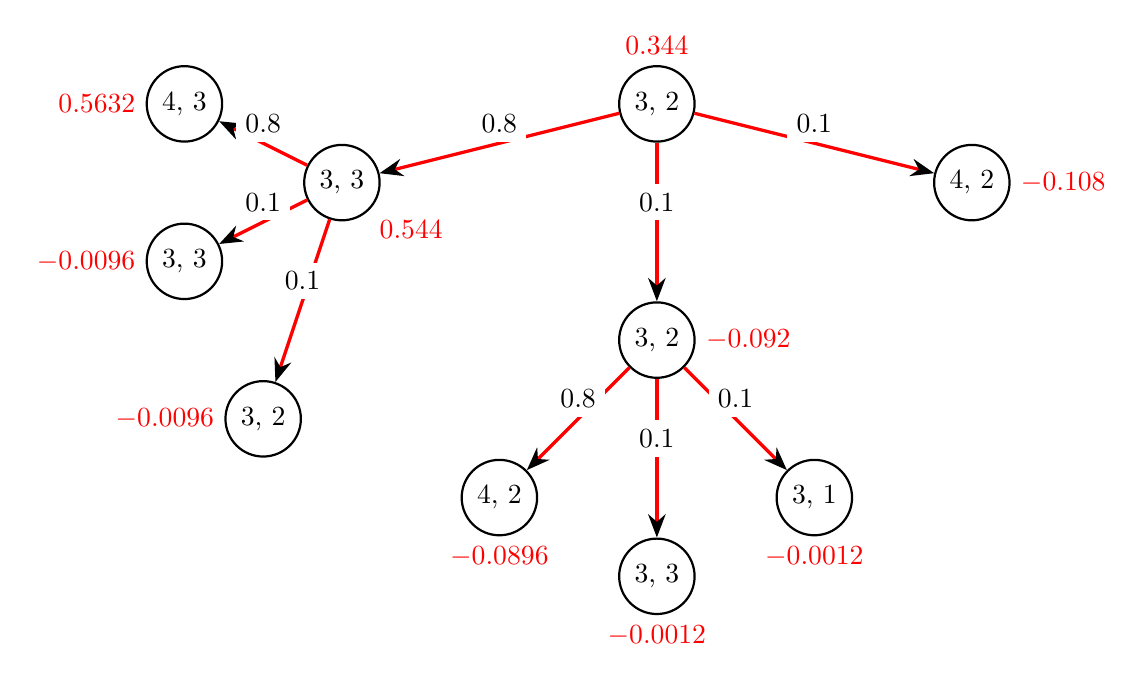
\begin{tikzpicture}
\begin{scope}[
    every node/.style={circle,thick,draw},
    every label/.append style={shape=rectangle,text=red}]
    \node (1) at (0, 0) [shape=circle,draw=black,fill=white,label=above:$0.344$] {3, 2};

    \node (2) at (-4, -1) [shape=circle,draw=black,fill=white,label=south east:$0.544$] {3, 3};

    \node (3) at (0, -3) [shape=circle,draw=black,fill=white,label=east:$-0.092$] {3, 2};

    \node (4) at (4, -1) [shape=circle,draw=black,fill=white,label=east:$-0.108$] {4, 2};

    % % 2nd node
    \node (5) at (-6, 0) [shape=circle,draw=black,fill=white,label=west:$0.5632$] {4, 3};
    \node (6) at (-6, -2) [shape=circle,draw=black,fill=white,label=west:$-0.0096$] {3, 3};
    \node (7) at (-5, -4) [shape=circle,draw=black,fill=white,label=west:$-0.0096$] {3, 2};

    % % 3rd node
    \node (8) at (-2, -5) [shape=circle,draw=black,fill=white,label=below:$-0.0896$] {4, 2};
    \node (9) at (0, -6) [shape=circle,draw=black,fill=white,label=below:$-0.0012$] {3, 3};
    \node (10) at (2, -5) [shape=circle,draw=black,fill=white,label=below:$-0.0012$] {3, 1};
\end{scope}

\begin{scope}[>={Stealth[black]},
              every node/.style={fill=white,rectangle,above},
              every edge/.style={draw=red,very thick}]
    \path [->] (1) edge node {0.8} (2);
    \path [->] (1) edge node {0.1} (3);
    \path [->] (1) edge node {0.1} (4);

    \path [->] (2) edge node {0.8} (5);
    \path [->] (2) edge node {0.1} (6);
    \path [->] (2) edge node {0.1} (7);

    \path [->] (3) edge node {0.8} (8);
    \path [->] (3) edge node {0.1} (9);
    \path [->] (3) edge node {0.1} (10);
\end{scope}
\end{tikzpicture}

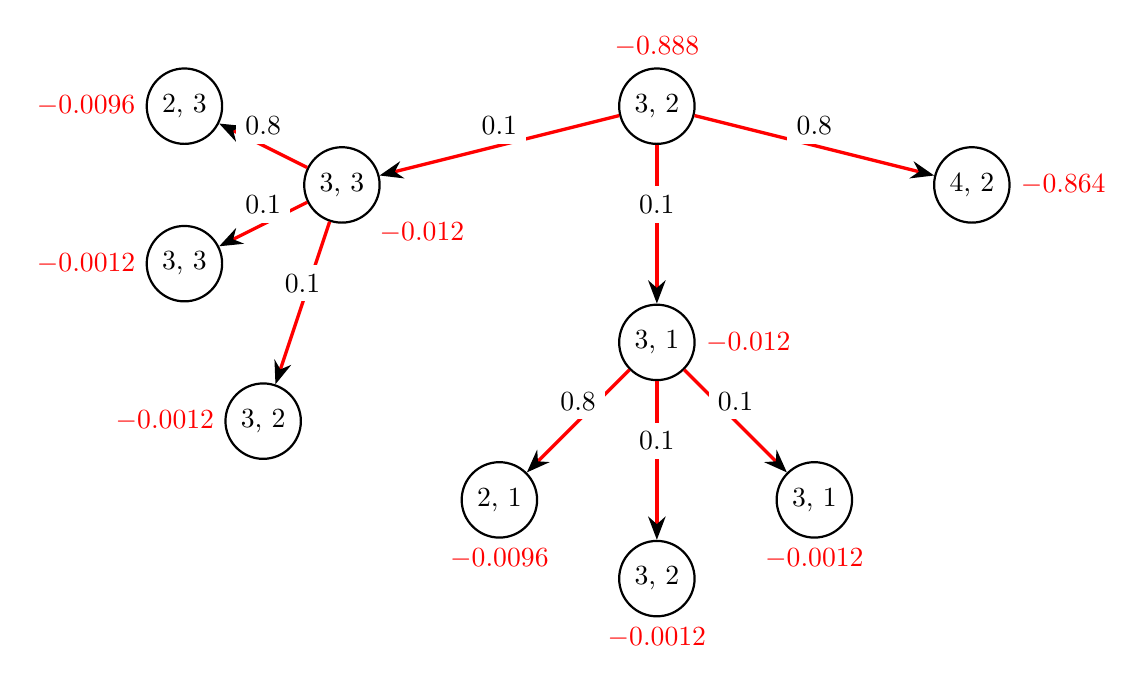
\begin{tikzpicture}
\begin{scope}[
    every node/.style={circle,thick,draw},
    every label/.append style={shape=rectangle,text=red}]
    \node (1) at (0, 0) [shape=circle,draw=black,fill=white,label=above:$-0.888$] {3, 2};

    \node (2) at (-4, -1) [shape=circle,draw=black,fill=white,label=south east:$-0.012$] {3, 3};

    \node (3) at (0, -3) [shape=circle,draw=black,fill=white,label=east:$-0.012$] {3, 1};

    \node (4) at (4, -1) [shape=circle,draw=black,fill=white,label=east:$-0.864$] {4, 2};

    % % 2nd node
    \node (5) at (-6, 0) [shape=circle,draw=black,fill=white,label=west:$-0.0096$] {2, 3};
    \node (6) at (-6, -2) [shape=circle,draw=black,fill=white,label=west:$-0.0012$] {3, 3};
    \node (7) at (-5, -4) [shape=circle,draw=black,fill=white,label=west:$-0.0012$] {3, 2};

    % % 3rd node
    \node (8) at (-2, -5) [shape=circle,draw=black,fill=white,label=below:$-0.0096$] {2, 1};
    \node (9) at (0, -6) [shape=circle,draw=black,fill=white,label=below:$-0.0012$] {3, 2};
    \node (10) at (2, -5) [shape=circle,draw=black,fill=white,label=below:$-0.0012$] {3, 1};
\end{scope}

\begin{scope}[>={Stealth[black]},
              every node/.style={fill=white,rectangle,above},
              every edge/.style={draw=red,very thick}]
    \path [->] (1) edge node {0.1} (2);
    \path [->] (1) edge node {0.1} (3);
    \path [->] (1) edge node {0.8} (4);

    \path [->] (2) edge node {0.8} (5);
    \path [->] (2) edge node {0.1} (6);
    \path [->] (2) edge node {0.1} (7);

    \path [->] (3) edge node {0.8} (8);
    \path [->] (3) edge node {0.1} (9);
    \path [->] (3) edge node {0.1} (10);
\end{scope}
\end{tikzpicture}

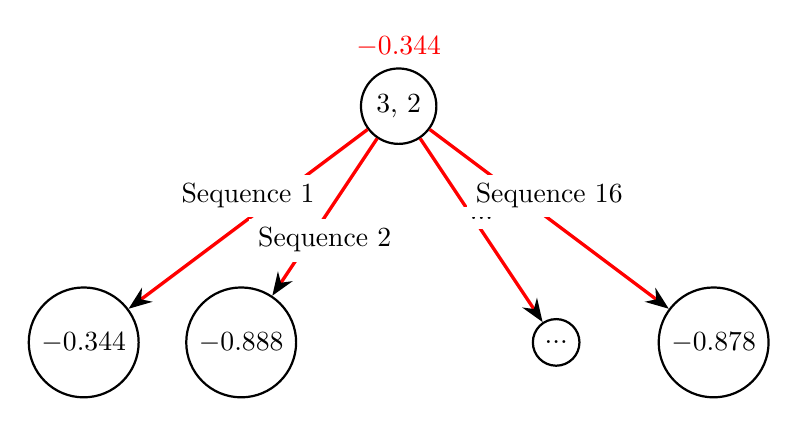
\begin{tikzpicture}
\begin{scope}[
    every node/.style={circle,thick,draw},
    every label/.append style={shape=rectangle,text=red}]
    \node (1) at (0, 0) [shape=circle,draw=black,fill=white,label=above:$-0.344$] {3, 2};

    \node (2) at (-4, -3) [shape=circle,draw=black,fill=white] {$-0.344$};

    \node (3) at (-2, -3) [shape=circle,draw=black,fill=white] {$-0.888$};

    \node (4) at (2, -3) [shape=circle,draw=black,fill=white] {...};

    \node (5) at (4, -3) [shape=circle,draw=black,fill=white] {$-0.878$};
\end{scope}

\begin{scope}[>={Stealth[black]},
              every node/.style={fill=white,rectangle,above},
              every edge/.style={draw=red,very thick}]
    \path [->] (1) edge node {Sequence 1} (2);
    \path [->] (1) edge node[below] {Sequence 2} (3);
    \path [->] (1) edge node {...} (4);
    \path [->] (1) edge node {Sequence 16} (5);

\end{scope}
\end{tikzpicture}
\end{document}
